\documentclass{llncs}
\usepackage{graphicx}
\usepackage{listings}

\begin{document}

\title{Linked Open Statistical Data API: requirements and design criteria}

\author{xxx ddd \and yyy sss}

\maketitle

\begin{abstract}

\end{abstract}

\section{Introduction}\label{sec:intro}

Recently, many governments, organisations and companies are opening up their data for others to reuse through \textit{Open Data} portals  \cite{Kalampokis:2011:IJWET}. These data can be exploited to create added value services, which can increase transparency, contribute to economic growth and provide social value to citizens \cite{Janssen:2012}.

A major part of open data concerns statistics (e.g. economical and social indicators) \cite{Capadisli:2013}. These data are often organised in a multidimensional way, where a measured fact is described based on a number of dimensions. In this case, statistical data are compared to data cubes. Thus, we onwards refer to statistical multidimensional data as \textit{data cubes} or just \textit{cubes}.

Linked data has been introduced as a promising paradigm for opening up data because it facilitates data integration on the Web \cite{Bizer:2009}. Concerning statistical data, the RDF data cube (QB) vocabulary enables modelling data cubes as linked data \cite{Cyganiak:2014:W3C}. In this way it facilitates their integration. Data provided using the QB vocabulary can be accessed using the existing machinery of Linked Data. However, skills and tooling for use of linked data (e.g. RDF, SPARQL) are less widespread than some other web technologies (e.g. JSON, REST). For example, there are many visualization libraries that consume data in JSON format (e.g D3.js, charts.js), while there are just a few that consume RDF and their functionality is limited. That's one of the reasons that there are not many application for linked data cubes [REF???].

Moreover, many portals that use the QB vocabulary often adopt different publishing practices \cite{KalampokisChallenges}, thus hampering their interoperability. As a result it is not easy to create generic software tools that operate across linked data cubes. Usually, case specific software are created which assume that linked data cubes are published only in a specific form. 

In this paper we describe the requirements and design criteria of an API that standardizes the interaction (i.e. input and output) with linked data cubes (aka Linked Open Statistical Data) in a way that facilitates the development of generic software. The API aims to exploit the advantages of linked data (e.g. easy data integration) but hide all the complexity. Specifically, it supports developers use linked statistical data stored in the form of an RDF Data Cube, while assuming minimal knowledge of linked data technologies. Moreover, the API offers a uniform way to access the underlying data by hiding any data discrepancies, thus enabling the development of generic software tools that operate across datasets. 

The rest of the paper is organized as follows ... +++

\section{Methodology}\label{sec:methodology}

In order to achieve the objectives of the paper we adopt the following methodology:
\begin{itemize}
\item Study the related work. We focus on: i) APIs that facilitate the interaction with data cubes and ii) data formats that can be exploited to represent the result (i.e. output) of the API. 
\item Collect user requirements from developers that currently create applications for linked data cubes. 
\end{itemize}

Currently, there exist many APIs that facilitate the interaction with data cubes. These APIs offer basic functionality that covers the cube's logical model, but they also support more advanced OLAP operations including aggregations, slicing, roll-up/drill-down etc. For example, the Oracle OLAP Java API \cite{ORACLEAPI} allows users to select, explore, aggregate, calculate, and perform other analytical tasks on data stored at Oracle data warehouse. Olap4j\footnote{http://www.olap4j.org} is another Java API for accessing data cubes, which is compatible with many OLAP servers (e.g. Mondrian, Palo and SAP Business Warehouse). It enables the browsing of meta-data including the cubes, dimensions, hierarchies and members in an schema. Olap4j also supports Multidimensional Expressions (MDX) that is the query language for OLAP.

There exist also some REST APIs with similar functionality. The Data Brewery\footnote{http://databrewery.org/} offers a set of Python tools, including a REST API, for processing and analysing data cubes stored at a relational data base (e.g. MySQL, PostgreSQL). Apache Lens\footnote{lens.apache.org} is another analytics platform that integrates Hadoop with traditional data warehouses (e.g. Apache Hive, Amazon Redshift). Lens provides a REST API to handle data cubes, that also supports ``OLAP Cube QL" - a high level SQL like language to query data organized as data cubes.

All the above APIs handle data cubes that are stored at traditional databases or data-warehouse. However, none of them can handle data cubes  stored as linked data using the QB vocabulary.  

<<<<<<< HEAD
The JSON-QB API purpose is to help users retrieve information to support visualizations and other applications. It can be easily done as its implementation fills the gap of a generic software interaction with every type of LOSD. Moreover, it retains the benefits of Linked Data such as data representation and integration, but hides most of the complexity of that for the majority of users. Next, we present an overview of the solution that was designed.

The architecture of the API is relatively simple as it is developed on the RDF Data Cube vocabulary and SPARQL using statistical data from the data cube structure. The implementation of JSON-API abolishes the need to implement different data access layers for each tool is created. In the traditional architecture data access layers had to be coded separately leading to additional costs. The JSON-API can be installed on top of any RDF repository and offers basic and advanced operations on RDF Data cubes while other kinds of database could be used, enabling flexibility and innovation.

Linked data is a good approach for standards-based publication of statistics on the web, but RDF and SPARQL are unfamiliar to many users. There are obstacles to uptake of this technology because it is perceived to be complicated. The aim of the API is to support a style of interaction that is familiar to web developers - delivering data in JSON format and using familiar styles of API call. Through SPARQL queries, JSON-API has full access at data cubes returning the asked data in the re-used format of JSON. Users can use JSON as input to the API for -get requests and receive data as output still in JSON format.
=======
Regarding the output of the REST APIs, JSON is an already successful and simple format. Existing REST APIs use some case-specific JSON responses, however JSON extension formats have already been proposed to model data cubes and linked data. Specifically, JSON-LD\footnote{https://json-ld.org} offers a method for encoding linked data using JSON. While, JSON-stat\footnote{https://json-stat.org/} is a JSON format for modelling statistical data (i.e. data cubes), however the structure is too complicated when it comes to simple visualizations (e.g. maps). Moreover, it has some limitations e.g. does not support pagination of results. 

Finally, to collect the user requirements, we established a continuous discussion with developers that currently create applications for linked data cubes. The discussion occurs within the EU funded project OpenGovIntelligence\footnote{http://www.opengovintelligence.eu/}, that aims to exploit linked data cubes for improving the public services. To facilitate the collection of requirements we organized a dedicated workshop at Manchester with participation of relevant developers. 


\section{Solution overview}\label{sec:overview}

A large part of statistical data is isolated, meaning that exists in different portals as different datasets. The technology of Linked data and RDF Data Cube vocabulary solves the problem of distributed data sources through their integration, creating interoperable linked statistical data portals. These portals are used for the design and creation of a Linked Open Statistical Data API.
 
The architecture of the API is developed in JSON format offering benefits which are not exist until now. The implementation of JSON-API abolishes the need to implement different data access layers for each tool is created. In the traditional architecture data access layers had to be coded separately leading to additional costs. The JSON-API can be installed on top of any RDF repository and offers basic and advanced operations on RDF Data cubes.
 
Moreover, using JSON for accessing RDF Stores is an easier way to build software applications. Developers need to know and use neither RDF Data Cube vocabulary nor expert programming skills at LOSD. They have full access at LOSD just using JSON, a much more common and understandable programming language. Through SPARQL queries, JSON-API has access at data cubes returning the asked data in the re-used format of JSON. By this way, all LOSD-related programming and its complexity is now hidden.

As figure 1 shows, JSON-API helps developers create custom applications according to their needs. JSON language is commonly re-used by many libraries offering data representation and visualization. +++
>>>>>>> 69e4a773d6fe3a7ad94ddeec13c046e1d6b51ecd

There are already methods available for downloading entire data cubes but people often want just small parts.  Whole cubes are often too big to be well-suited to interactive applications, and if the data updates frequently, then it's important for people to be able to retrieve up-to-date extracts of the data, rather than keeping their own copies of full datasets up to date. JSON-QB API implementation allows developers through JSON to take exactly the data that want.
 
In addition, we want to standardise the API specification and try to get broad support for it, so that many data publishers can provide data in a compatible way, making tools interoperable. As well as making data easier to consume, using the API as the main method of delivering machine readable extracts of data would remove or greatly reduce the need for data publishers to provide public SPARQL endpoints. By this way cost can be reduced and reliability of open services could be improved.

\begin{figure}
  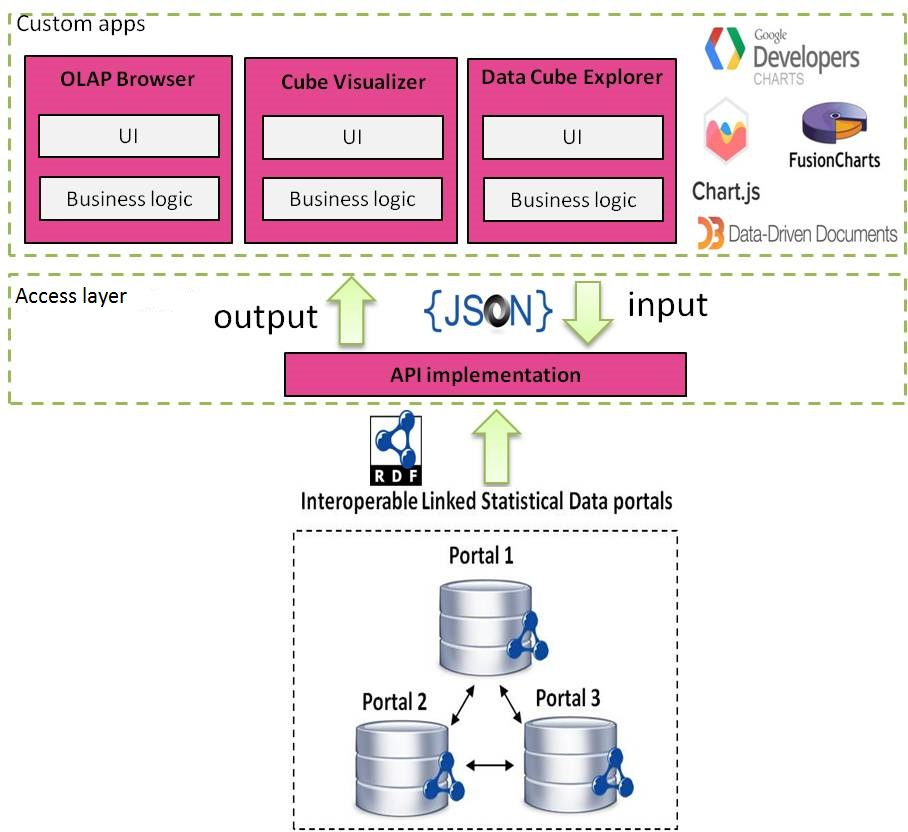
\includegraphics{images/overview.jpg}
\caption{Solution overview}
\label{fig:overview}
\end{figure}


\section{Requirements and design criteria}\label{sec:reqs}

This section presents the requirements and design criteria related to the Linked Open Statistical Data API.

\subsection{Explore data cubes}

The linked data web currently contains many published data cubes and their number still increases. Obviously there is a need to search for cubes based on some criteria. For example get cubes that measure unemployment, or get cubes that for Greece. The criteria can be even more complex e.g. get cubes about unemployment in Greece after 2010. This functionality will enable web developers create advanced exploring functionality among cubes that exist even at different RDF stores.

This functionality can be extended to support not only user specified criteria, but also support the automatic search of cubes that could be processed together. For example, search for cubes that are compatible for statistical analysis, or for browsing. The compatibility criteria is still an open issue and is under discussions.

\subsection{Explore data cube structure}
GET dataset-metadata

GET dimensions

GET attributes

GET measures

GET dimension-values

GET attribute-values

GET dimension-levels

mazi me to epomeno?


\subsection{Slicing or filtering}
There are already methods available for downloading entire data cubes but people often want just small parts.  Whole cubes are often too big to be well-suited to interactive applications, and if the data updates frequently,  then it's important for people to be able to retrieve up-to-date extracts of the data, rather than keeping their own copies of full datasets up to date

Need to know about structure to subset the observations. In order not to return everything, need to subset

Filtering

don't necessarily need a n-array/ tabular response - array of observations is sufficient. can always get back to the table

GET slice
GET table


\subsection{Data integration}

Retain the benefits of Linked Data for behind the scenes data representation and integration, but hide most of the complexity of that for the majority of users

Merging 

json-ld representation is sufficient for query and response format

\subsection{Data representation agnostic}
we want to standardise the API specification and try to get broad support for it, so that many data publishers can provide data in a compatible way, making tools interoperable.  So the API has to be generic enough to be widely applicable.


\subsection{Easy of use by web developers}
purpose is to help users retrieve information to support visualisations and other applications.
the well-defined structure of RDF Data Cube means that the API can be relatively simple
linked data is a good approach for standards-based publication of statistics on the web, but RDF and SPARQL are unfamiliar to many users and there are obstacles to uptake of this technology because it is perceived to be complicated. our aim is to support a style of interaction that is familiar to web developers. Delivering data in JSON format and using familiar styles of API call 


\subsection{Performance}
It will be easier to support efficient caching of API responses than of arbitrary SPARQL queries

Ordering \& paging


\subsection{Extensibility}
while our initial implementations are building on top of underlying RDF databases, other kinds of database could be used, enabling flexibility and innovation. 

Multilinguality

API vs language

\subsection{Other}


as well as making data easier to consume, using the API as the main method of delivering machine readable extracts of data would remove or greatly reduce the need for data publishers to provide public SPARQL endpoints, so reducing cost and improving reliability of open online services

aggregations


possible example for slice/ observation-selection query:
\begin{verbatim} 
{ 
  "jqql:dataset": "scot:home-care-clients",
  "jqql:filter": {
"dimension:gender": "gender:male",
   "dimension:age": { "jqql:greater-than": 50 }
  },
  "jqql:order": {
    "dimension:refPeriod": { "jqql:order-predicate": "ui:sortPriority", "jqql:direction": "jqql:asc"}
  },
  "jqql:page": {
    "jqql:limit": 10,
    "jqql:offset": 0
  }
}
\end{verbatim}

output:
\begin{verbatim} 
{ "observations": [ 
	{ "Average Cost": "1182", 
   	  "Date": "1-1-2013", 
	  "Day": "Tuesday", 
	  "Number of crashes": "5",
	  "Time": "No available time",
      "Total Cost": "5908", 
	  "@id": http://id.mkm.ee/observation/1" }, 
	{ "Average Cost": "400",
	  "Date": "1-1-2013",
	  "Day": "Tuesday",
	  "Number of crashes": "1",
	  "Time": "24:00",
 	  "Total Cost": "400",
	  "@id": "http://id.mkm.ee/observation/2" }
]}
\end{verbatim}

\section{Implementation}\label{sec:impl}

\section{Conclusion}\label{sec:conclusion}


%\begin{acknowledgements}
%If you'd like to thank anyone, place your comments here
%and remove the percent signs.
%\end{acknowledgements}

\bibliographystyle{splncs03}


\bibliography{qbbibfile}   % name your BibTeX data base


\end{document}


